\documentclass[a4paper,ngerman]{scrartcl}

\usepackage{amsmath}
\usepackage{amsfonts}
\usepackage{amssymb}
\usepackage[utf8]{inputenc}
\usepackage{graphicx}
\usepackage[ngerman]{babel}
\usepackage{hyperref}
\usepackage{float}
\usepackage{caption}
\usepackage{subcaption}
\usepackage{multirow}  %for tables
\usepackage{icomma} % Handle german comma as decimal point in numbers
\usepackage{units,siunitx} % Write units with correct spacing
\usepackage{upgreek} % provide non-italic greek letters
\usepackage{url}
\usepackage{booktabs}
%\usepackage{subfig}

% Formatting of table & figure captions
\captionsetup{font={sf,footnotesize},labelfont=bf,textfont=sl,skip=6pt}
\setlength{\abovecaptionskip}{6pt}
\setlength{\belowcaptionskip}{0pt}

\title{Magnetisierung\\Versuchsauswertung}
\date{\today}
\author{Michel Rausch, Michael Eliachevitch}

\begin{document}

\maketitle
\tableofcontents
\newpage

\section{Versuchsvorbereitung}








\section{Versuchsauswertung}



\subsection{Kalibrierung des SQUIDs}


\subsubsection*{Mit der Kalibrierungsspule}

Ein Kupferzylinder ($\rm{Durchmesser} = \SI{0.7}{\centi \meter}$,  Höhe $ = \SI{0.7}{\centi \meter}$) mit mit der Spule wurde auf den Probenhalter geschraubt. 
Der Halter wurde so im Magnetfeld platziert, dass die Spule nach oben gerichtet war.
Damit wurde sichergestellt, dass die Proben später in einer möglichst gleichen und somit vergleichbaren Position befanden.
Zehn Messwerte wurden genommen, für unterschiedliche Spulenströme. 
Diese sind in Tabelle \ref{tab:Kalibrierung-Magnetfeld} aufgelistet.
Das Magnetfeld des SQUIDs wurde nach dem Biot-Savartschem Gesetz [\ref{ref:mappe}] berechnet mit

\begin{equation}
B_{\mathrm{Spule}} = \mu_{\rm{0}} \cdot \frac{R^2}{2 x^3} ~.
\end{equation}

Mit der absoluten magnetischen Permeabilität $\mu_{\rm{0}}$, dem Abstand der Spule zum SQUID $d = \SI{1.4}{\centi \meter}$ und dem Radius der Spule $R = \SI{0.35}{\centi \meter} $.
Der Abstand der Spule zum SQUID schien beim tatsächlichem Aufbau signifikant größer zu sein, als bei der Versuchsbeschreibung angegeben,
dennoch wurde mit dem Wert aus der Mappe gerechnet.


\begin{table}[tb!]
\centering
\caption[Kalibrierung]{\textbf{Messwerte zur Kalibrierung des SQUIDs.} }
\begin{tabular}{ccc}
\toprule
Spulenstrom	in mA &	SQUID-Spannung in mV	\\
\midrule
0	&	19	\\
40	&	27	\\
80	&	29	\\
119	&	42	\\
147	&	42	\\
180	&	52	\\
209	&	40	\\
235	&	65	\\
315	&	58	\\
360	&	66	\\
\bottomrule
\end{tabular}
\label{tab:Kalibrierung-Magnetfeld}
\end{table}

In Abbildung \ref{fig:Kalibrierung-Magnetfeld} ist die Messreihe mit zugehörigem linearem Fit mit Python dargestellt.
Man erkennt, dass sehr geringe Magnetfeldstärken in der Größenordnung eines Mikroteslas gemessen wurden.
Das SQUID ist also ein äußerst empfindliches Messgerät.
Die lineare Regression ergab

\begin{equation}
\label{eq:B(U_SQUID)}
B = \SI{18+-3}{\micro \tesla \per \mV} \cdot U_{\mathrm{SQUID}} - \SI{0.3+-0.1}{\micro \tesla} ~.
\end{equation}

%U_{\mathrm{SQUID}} = \SI{46+-7}{\mV \per \micro \tesla} \cdot B + \SI{22+-4}{\mV} ~.

\begin{figure}
\centering
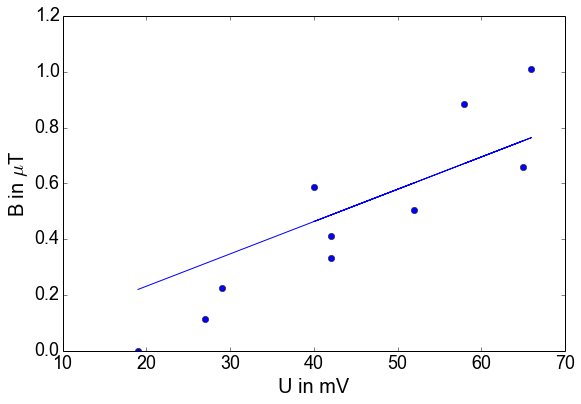
\includegraphics[width=0.8\textwidth]{abbildungen/kalibrierung_spule.png}
\caption[Kalibrierung des SQUIDs mit Spule]{\textbf{Kalibrierung des SQUIDs mit Spule.} Für unterschiedliche Ströme durch die Spule wurde die resultierende Spannung am SQUID gemessen. Die Messwerte streuten stark, daher war ein hoher Fehler zu erwarten.}
\label{fig:Kalibrierung-Magnetfeld}
\end{figure}




\subsubsection*{Mit der Nickelprobe}

Eine Nickelprobe mit dem Ausmaßen $\SI{5}{\mm} \times \SI{5}{\mm} \times \SI{0.1}{\mm}$ wurde auf den Probenhalter geschraubt.
Aus ihrem Volumen und der spezifischen Magnetisierung von Nickel [\ref{ref:mappe}]
\begin{equation}
\sigma = \SI{55.09}{\ampere \square \meter \per \kg} ~,
\end{equation}
sowie der Masse der Probe 
\begin{equation}
m = \SI{0.0202}{\gram} ~,
\end{equation}
wurde das maximale magnetische Moment der Nickelprobe 

\begin{equation}
\mu_{\mathrm{Ni}} = \SI{1.11}{\mA \square \meter}
\end{equation}

bestimmt. Die Probe wurde magnetisiert, bei einem maximalem Strom durch die Magnetspulen von
\begin{equation}
I_{\mathrm{Spule}} = \SI{1.168}{\ampere} ~.
\end{equation}

Einmal wurde die Probe senkrecht zum Magnetfeld orientiert, das andere Mal parallel.
Bei einer senkrechten Orientierung betrug die Spannung am SQUID ohne Probe 
\begin{equation}
U_{\mathrm{ohne Probe},\perp} = \SI{83}{mV} ~.
\end{equation}
Mit der Probe stieg die Spannung auf
\begin{equation}
U_{\mathrm{mit Probe},\perp} = \SI{970}{mV} ~.
\end{equation}

Die Spannungsdifferenz wird durch die Probe verursacht und wird in 
Gleichung \eqref{eq:B(U_SQUID)} als Argument verwendet, um das Magnetfeld zu bestimmen. 

\begin{equation}
B_{\mathrm{mit Probe},\perp} = \SI{16+-3}{mT} ~.
\end{equation}


Als die Probe parallel zum Magnetfeld war ergaben sich analog
\begin{equation}
U_{\mathrm{ohne Probe},\parallel} = \SI{70}{mV} ~,
\end{equation}
\begin{equation}
U_{\mathrm{mit Probe},\parallel} = \SI{1620}{mV} ~,
\end{equation}
\begin{equation}
B_{\parallel} = \SI{28+-5}{mT} ~.
\end{equation}

Im Vergleich sieht man, dass die Nickelprobe bei parallelem Einbau stärker magnetisiert worden ist.
Für das Magnetfeld gilt mit dem Abstand der probe zum SQUID [\ref{ref:mappe}]
\begin{equation}
B = \frac{\mu_{\rm{0}} \mu }{2 \uppi x^3} ~.
\end{equation}

Daraus folgt
\begin{equation}
\label{eq:mu(B))}
\mu = \frac{2 \uppi B x^3 }{\mu_{\rm{0}}} ~.
\end{equation}

Die Magnetischen Momente sind dann für den senkrechten Einbau
\begin{equation}
\mu_{\perp} = \SI{0.22+-0.04}{\mA \square \meter} ~,
\end{equation}

und für den parallelen
\begin{equation}
\mu_{\parallel} = \SI{0.38+-0.07}{\mA \square \meter} ~.
\end{equation}

In beiden Fällen ist das magnetische Moment, und somit die Magnetisierung, geringer als die maximal mögliche.
Dies ist mit der Stärke des Magnetfeldes zu erklären.
Das vorhandene Netzteil und die Spule konnten nur Magnetfeldstärken liefern die nicht zur Sättigung genügten.
Da die Probe nicht vollständig aufmagnetisiert wurde, kann von einem linearem Verhältnis der Magnetisierung zur Magnetfeldstärke ausgegangen werden.

Aus Gleichungen \eqref{eq:B(U_SQUID)} und \eqref{eq:mu(B))} zusammen folgt der Zusammenhang zwischen Magnetisierung und Spannung am SQUID

\begin{equation}
\mu(U_{\mathrm{SQUID}}) = \frac{2 \uppi  x^3 }{\mu_{\rm{0}}} \cdot  \left( \SI{18+-3}{\micro \tesla \per \mV}  \cdot U_{\mathrm{SQUID}} - \SI{0.3+-0.1}{\micro \tesla} \right) ~.
\end{equation}

Die Kalibrierung der Spule war ungenau, daher war ein hoher statistische Fehler zu erwarten.
Zudem war der Abstand der Probe zum SQUID wahrscheinlich größer als angegeben.
Das Verhalten der Probe unter einem Magnetfeld entspricht jedoch den Erwartungen. 

\subsection{Magnetisierungsmessungen}


\subsubsection{Terbiumprobe bei senkrechtem Einbau}

\subsubsection*{Messung mit im Nullfeld gekühlter Probe ohne Magnetisierung}

Die Probe wurde in die Spule montiert und abgekühlt.
Es wurde kein Magnetfeld angelegt.
Die Messung begann, als die Temperatur unter \SI{80}{K} gesunken war.
Die Probe wurde bei das SQUID eingebaut und die Kühlung wurde unterbrochen.
Um den Aufwärmvorgang zu beschleunigen wurde Pressluft eingeleitet.
Die vorhandene Software protokollierte die Spannungen am SQUID und die zugehörige Temperatur.
In Abbildung \ref{fig:Tb_sr_0} ist die Messreihe gezeigt.


\begin{figure}
\centering
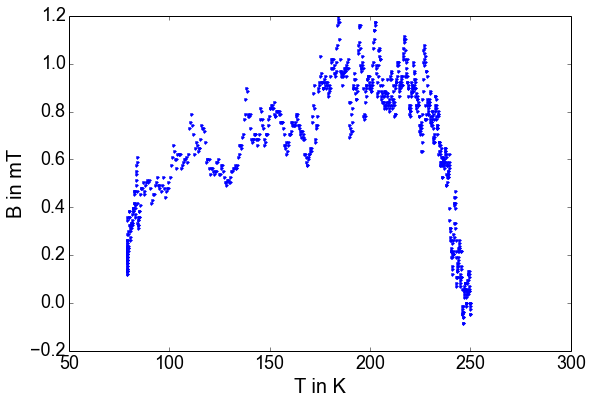
\includegraphics[width=0.6\textwidth]{abbildungen/Tb_sr_0.png}
\caption[Terbiumprobe senkrecht bei Nullfeld]{\textbf{Terbiumprobe senkrecht bei Nullfeld gekühlt, Rohdaten.} Die Spannung am SQUID ist über die Temperatur aufgetragen.}
\label{fig:Tb_sr_0}
\end{figure}

Über einen Anteil von 10~\% wurde eine lokale Regression (LOWESS) durchgeführt, wie in Abbildung \ref{fig:Tb_sr_0_glatt} gezeigt ist.
Um die Curietemperatur zu bestimmen wurde mit den  der Gradient gebildet.
Das sichtbare Minimum befindet sich an der Temperatur

\begin{equation}
T_{\rm{C}} = \SI{244}{\K} ~.
\end{equation}


\begin{figure}
\centering
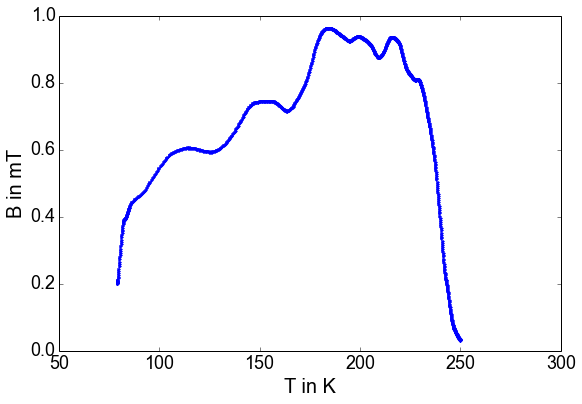
\includegraphics[width=0.5\textwidth]{abbildungen/Tb_sr_0_glatt.png}
\caption[Terbiumprobe senkrecht bei Nullfeld]{\textbf{Terbiumprobe senkrecht bei Nullfeld gekühlt, geglättet mit LOWESS.} Die Spannung am SQUID ist über die Temperatur aufgetragen, wie in Abb. \ref{fig:Tb_sr_0}. Mit der Python-Funktion LOWESS wurde eine lokale Regression über 10~\% der Daten durchgeführt.}
\label{fig:Tb_sr_0_glatt}
\end{figure}


\begin{figure}
\centering
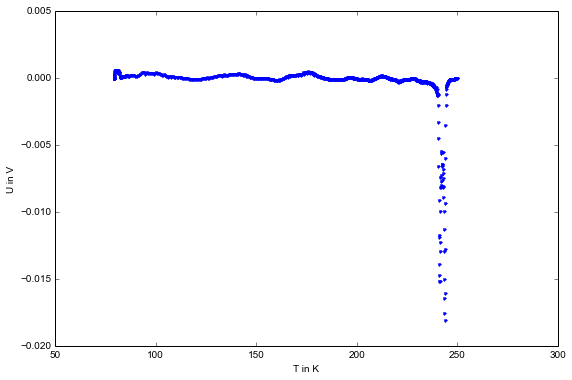
\includegraphics[width=0.6\textwidth]{abbildungen/Tb_sr_0_grad.png}
\caption[Terbiumprobe senkrecht bei Nullfeld]{\textbf{Terbiumprobe senkrecht bei Nullfeld gekühlt, geglättet und Gradient gebildet.} Die Spannung am SQUID ist über die Temperatur aufgetragen. Ein Minimum ist an der Curietemperatur zu erkennen.}
\label{fig:Tb_sr_0_grad}
\end{figure}

\subsubsection*{Messung mit im Nullfeld gekühlter Probe mit Magnetisierung bei tiefer Temperatur und einem magnetfeld mit \SI{15}{mT}}

Die Probe wurde nach dem Erwärmen wieder gekühlt auf unter \SI{80}{K}.
Dabei wurde kein Magnetfeld angelegt.
Erst als die Probe abgekühlt war, wurde die Spule aktiviert, sodass ein Magnetfeld mit \SI{15}{mT} vorhanden war.
Der Strom durch die Spule betrug dabei etwa \SI{150}{\mA}.
Die Umrechnung vom Spulenstrom auf das Magnetfeld konnte mit 
\begin{equation}
10 \cdot B/\mathrm{mT} = I /\mathrm{mA}
\end{equation} 
genähert werden. 
Die Umrechnung war genauer gegeben, aber da sich der Strom nicht genau einstellen lies, konnte auf höhere Genauigkeit verzichtet werden.


\begin{figure}
\centering
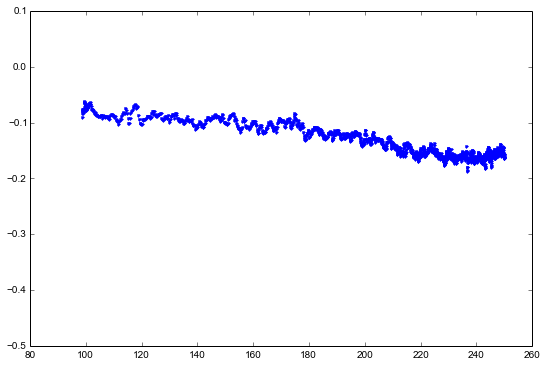
\includegraphics[width=0.6\textwidth]{abbildungen/Tb_sr_0_mit.png}
\caption[Terbiumprobe senkrecht bei Nullfeld]{\textbf{Terbiumprobe senkrecht bei Nullfeld gekühlt, Rohdaten.} Die Spannung am SQUID ist über die Temperatur aufgetragen.}
\label{fig:Tb_sr_0_mit}
\end{figure}

Die Messergebnisse sind in Abbildung \ref{fig:Tb_sr_0_mit} gezeigt. 
Der Gradient wurde aus den geglätteten Daten gebildet, wie in Abbildung \ref{fig:Tb_sr_0_grad_mit} dargestellt ist. 
Es ist kein ausgewiesenes Minimum zu erkennen, daher konnte keine Curietemperatur bestimmt werden.


\begin{figure}
\centering
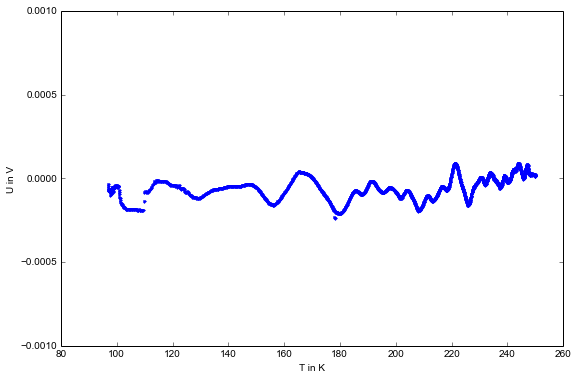
\includegraphics[width=0.6\textwidth]{abbildungen/Tb_sr_0_grad_mit.png}
\caption[Terbiumprobe senkrecht bei Nullfeld]{\textbf{Terbiumprobe senkrecht bei Nullfeld gekühlt, geglättet und Gradient gebildet} Die Spannung am SQUID ist über die Temperatur aufgetragen. Es wurden über über 25~\% der Daten mittels LOWESS geglättet. Es ist kein Minimum zu erkennen und somit keine Curietemperatur ermittelbar.}
\label{fig:Tb_sr_0_grad_mit}
\end{figure}



\subsubsection*{Messung mit im Feld gekühlter Probe bei \SI{15}{mT}}


Das Magnetfeld wurde angestellt, bevor die Kühlung begann. 
Die Probe wurde bei aktivem Magnetfeld gekühlt. 
Gemessen wurde wie vorhin beim Erwärmen.
Hier traten einige Sprünge auf, wie in Abbildung \ref{fig:Tb_sr_15} zu sehen ist. 
Die Sprünge wurden nach Augenmaß korrigiert, aber da viele Unstetigkeiten im interessanten Bereich um die Curietemperatur auftraten,
konnte die Cuietemperatur nur schwer ermittelt werden.
Sie konnte dennoch identifiziert werden mit 

\begin{equation}
T_{\rm{C}} = \SI{235}{\K} ~.
\end{equation}


\begin{figure}
\centering
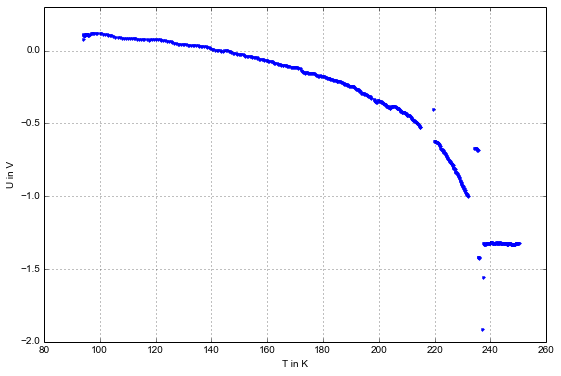
\includegraphics[width=0.6\textwidth]{abbildungen/Tb_sr_150.png}
\caption[Terbiumprobe senkrecht bei 15mT]{\textbf{Terbiumprobe senkrecht im Feld ($B = \SI{15}{mT}$) gekühlt, Rohdaten.} 
Die Spannung am SQUID ist über die Temperatur aufgetragen. 
Da die Messwerte stark sprangen mussten die Unstetigkeiten nach Augenmaß korrigiert werden.
Insbesondere an der interessanten Stelle um die Curietemperatur traten viele Sprünge auf.}
\label{fig:Tb_sr_15}
\end{figure}




\begin{figure}
\centering
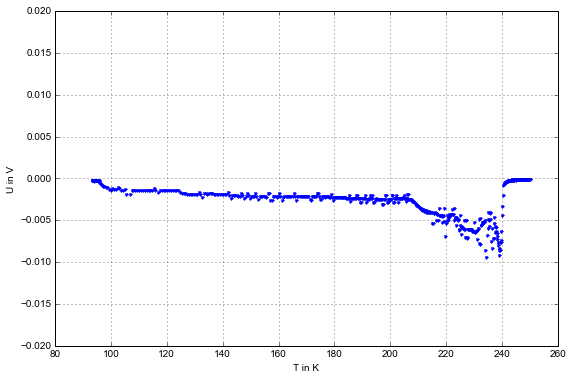
\includegraphics[width=0.6\textwidth]{abbildungen/Tb_sr_150_grad.png}
\caption[Terbiumprobe senkrecht bei Nullfeld]{\textbf{Terbiumprobe senkrecht im Feld ($B = \SI{15}{mT}$) gekühlt, geglättet und Gradient gebildet} 
Die Spannung am SQUID ist über die Temperatur aufgetragen. 
Es ist ein Minimum zu erkennen und somit eine Curietemperatur ermittelbar.
Die Sprünge gestalteten die Auswertung dieses Minimums schwierig.}
\label{fig:Tb_sr_15_grad}
\end{figure}



\subsubsection{Terbiumprobe bei parallelem Einbau}

Die Terbiumprobe wurde mit paralleler Ausrichtung auf den Probenhalter geschraubt. 
Ein Magnetfeld mit der vorgegebenen Feldstärke wurde angelegt und die Probe gekühlt.
War die Probe ausgekühlt, so wurde sie in den SQUID geführt.

\subsubsection*{Messung mit im Feld gekühlter Probe bei \SI{5}{mT}}

Außer einiger Abweichungen am Anfang der Messung ist der erwartete Verlauf in Abbildung \ref{fig:Tb_p_5} widergespiegelt.
Ein Minimum ist in der Steigung (Abb. ) eindeutig erkennbar und befindet sich an der Temperatur

\begin{equation}
T_{\mathrm{C}} = \SI{227}{\K} ~.
\end{equation}



\begin{figure}
\centering
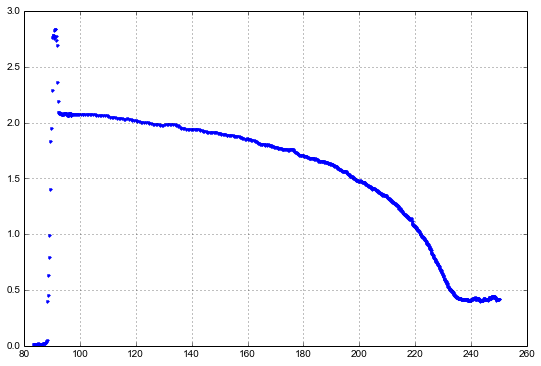
\includegraphics[width=0.6\textwidth]{abbildungen/Tb_p_5.png}
\caption[Terbiumprobe parallel bei 5mT]{\textbf{Terbiumprobe senkrecht im Feld ($B = \SI{5}{mT}$) gekühlt, Rohdaten.} 
Die Spannung am SQUID ist über die Temperatur aufgetragen. }
\label{fig:Tb_p_5}
\end{figure}
\begin{figure}
\centering
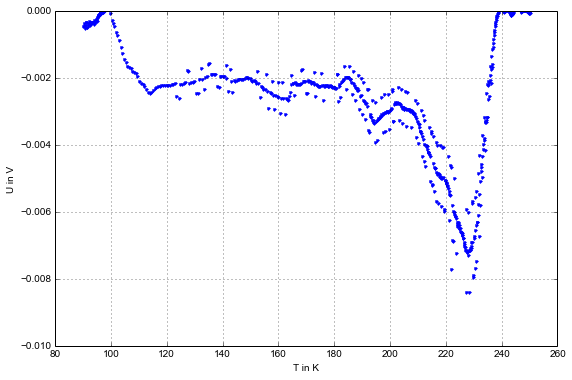
\includegraphics[width=0.6\textwidth]{abbildungen/Tb_p_5_grad.png}
\caption[Terbiumprobe parallel bei 5mT]{\textbf{Terbiumprobe senkrecht im Feld ($B = \SI{5}{mT}$) gekühlt, geglättet und Gradient gebildet} 
Die Spannung am SQUID ist über die Temperatur aufgetragen. 
Es ist ein Minimum zu erkennen und somit eine Curietemperatur ermittelbar.
Alle Messwerte über $T =\Si{90}{K}$ wurden ausgeblendet.
\label{fig:Tb_p_5_grad}
\end{figure}


\subsubsection*{Messung mit im Feld gekühlter Probe bei \SI{10}{mT}}

Der erwartete Verlauf in Abbildung \ref{fig:Tb_p_5} widergespiegelt.
Ein Minimum ist in der Steigung (Abb. ) eindeutig erkennbar und befindet sich an der Temperatur

\begin{equation}
T_{\mathrm{C}} = \SI{228}{\K} ~.
\end{equation}



\begin{figure}
\centering
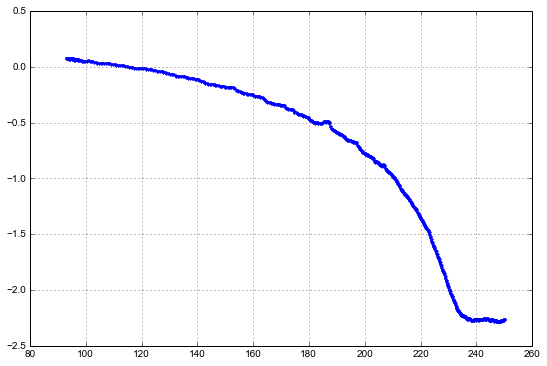
\includegraphics[width=0.6\textwidth]{abbildungen/Tb_p_10.png}
\caption[Terbiumprobe parallel bei 10mT]{\textbf{Terbiumprobe parallel im Feld ($B = \SI{10}{mT}$) gekühlt, Rohdaten.} 
Die Spannung am SQUID ist über die Temperatur aufgetragen. }
\label{fig:Tb_p_10}
\end{figure}

\begin{figure}
\centering
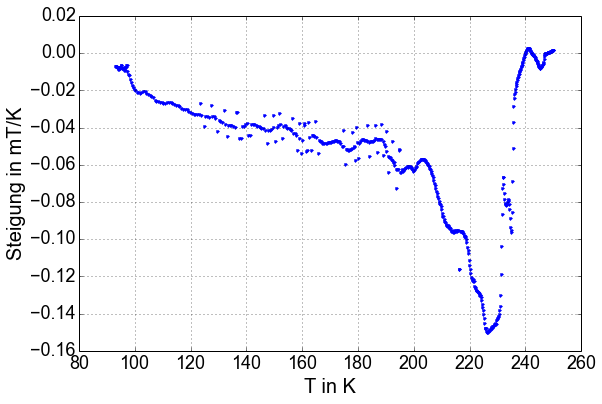
\includegraphics[width=0.6\textwidth]{abbildungen/Tb_p_10_grad.png}
\caption[Terbiumprobe parallel bei 10mT]{\textbf{Terbiumprobe parallel im Feld ($B = \SI{10}{mT}$) gekühlt, geglättet und Gradient gebildet} 
Die Spannung am SQUID ist über die Temperatur aufgetragen. 
Es ist ein Minimum zu erkennen und somit eine Curietemperatur ermittelbar.
\label{fig:Tb_p_10_grad}
\end{figure}


\subsubsection*{Messung mit im Feld gekühlter Probe bei \SI{15}{mT}}

Der erwartete Verlauf ist in Abbildung \ref{fig:Tb_p_5} widergespiegelt.
Ein Minimum ist in der Steigung (Abb. ) eindeutig erkennbar und befindet sich an der Temperatur

\begin{equation}
T_{\mathrm{C}} = \SI{227}{\K} ~.
\end{equation}

\begin{figure}
\centering
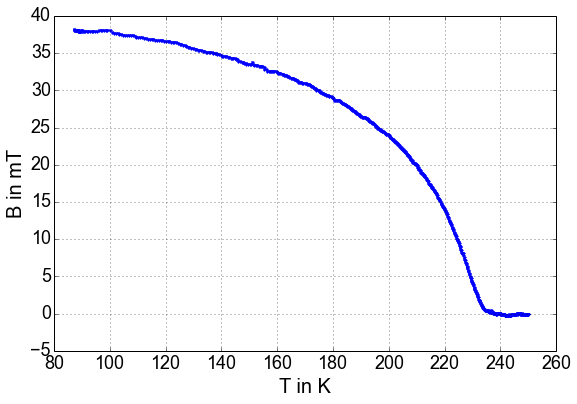
\includegraphics[width=0.6\textwidth]{abbildungen/Tb_p_15.png}
\caption[Terbiumprobe parallel bei 15mT]{\textbf{Terbiumprobe parallel im Feld ($B = \SI{15}{mT}$) gekühlt, Rohdaten.} 
Die Spannung am SQUID ist über die Temperatur aufgetragen. }
\label{fig:Tb_p_10}
\end{figure}

\begin{figure}
\centering
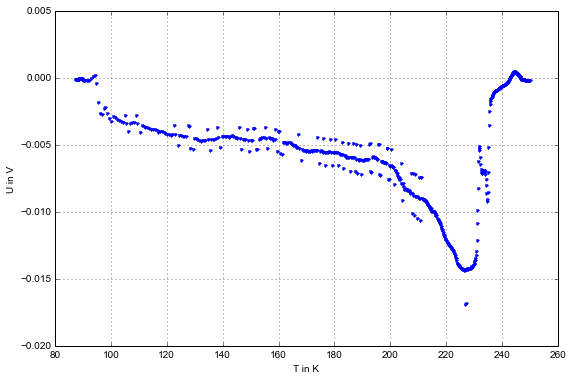
\includegraphics[width=0.6\textwidth]{abbildungen/Tb_p_15_grad.png}
\caption[Terbiumprobe parallel bei 15mT]{\textbf{Terbiumprobe parallel im Feld ($B = \SI{15}{mT}$) gekühlt, geglättet und Gradient gebildet} 
Die Spannung am SQUID ist über die Temperatur aufgetragen. 
Es ist ein Minimum zu erkennen und somit eine Curietemperatur ermittelbar.}
\label{fig:Tb_p_10_grad}
\end{figure}

\subsubsection{Vergleich}




\begin{table}[tb!]
\centering
\caption[Vergleich]{\textbf{Vergleich der Messergebnisse .} }
\begin{tabular}{ccc}
\toprule
Probe	&	T_{\mathrm{C}}	\\
\midrule
Tb senkrechter Einbau ohne Magnetisierung bei Nullfeld
\bottomrule
\end{tabular}
\label{teb:vergleich}
\end{table}








\subsubsection{Gadoliniumprobe}

\subsubsection*{Messung mit im Feld gekühlter Probe bei \SI{100}{mT}}







\section{Quellen}
\begin{enumerate}
\item Vorbereitungsmappe.\label{ref:mappe}
\item \url{http://hydrogen.physik.uni-wuppertal.de/hyperphysics/hyperphysics/hbase/solids/squid.html} (18.1.2015).\label{ref:wuppertal}
\item \url{http://jsq.apps-1and1.net/category/information/what-is-a-squid/} (18.1.2015).
\label{ref:jsq}
\end{enumerate}



\end{document}
